\section{Case Study of SDP: A Trial of Day-ahead TDP}\label{sec:TDP}

While pricing algorithms are essential to SDP research, in practice such algorithms must be able to function within an ISP network. In this section, we discuss the design and results of a trial of Section \ref{sec:dayahead}'s day-ahead time-dependent pricing (TDP) to highlight some ways in which implementability concerns can influence the development of pricing algorithms. We examine some important system and user interface design principles that were used in developing the prototype of this system, called TUBE, and finally present some trial results that illustrate how these elements can come together in practice. While some SDP trials have been conducted in the past, e.g., the Berkeley INDEX project in the 1990s \cite{INDEX}, the design of this TUBE pilot trial illustrates the way new factors such as smartphones' computing capabilities affect SDP's feasibility.

%Economic models for and system design for enabling dynamic pricing, such as time-dependent pricing (TDP), smart market auctions, sponsored access. Developing a control-feedback loop between the network core and end-devices (i.e., demand-response). Need for new usage accounting and signaling protocols. User interface design factors for smart pricing. Results from field trials of TDP systems.

\subsection{Model Considerations}

Most forms of dynamic pricing, in which prices must be determined in (near) real-time, require the prices to adapt based on users' behavior. For instance, users' perception of the prices offered may change over time, and demographically distinct user populations may react differently to the same set of prices (e.g., teenagers versus businessmen). Offering dynamic pricing thus requires that the ISP first estimate its users' behavior and then use this to inform its choice of prices. In the case of time-dependent pricing, such estimates are particularly important. The basic philosophy of TDP is that by offering lower prices at less congested times, an ISP incentivizes users to shift some of their usage from more expensive, congested times to less congested times. Users' demand over the day is thus even-ed out, with peak usage decreasing; this decrease in peak usage then reduces ISPs' need to over-provision capacity for their peak demand. While lower prices would effectively encourage users to shift their demand, thus reducing costs, ISPs would also lose a large amount of revenue if the prices were too low. Moreover, users might shift their usage too much, and end up creating a new peak period during the discounted times.

In practice, these estimates of user behavior must take into account the available information that the ISP can collect from its users. For instance, TUBE's TDP algorithms, discussed in Section \ref{sec:dayahead}, use only \emph{aggregate usage data}, that is, the total usage volume on the network at different times, in order to estimate user behavior and calculate the prices. This approach has the following benefits:
\begin{itemize}
\item
\emph{Scalability:} Since only aggregate usage is recorded and used in the algorithms \cite{ha2012tube}, we can scale up the user behavior and price computations to multiple users and multiple applications. The algorithm complexity does not increase with the number of users contributing to the aggregate usage totals.
\item
\emph{User privacy:} The amount of traffic that an individual consumes for different applications can be sensitive information (e.g., unusually large amounts of streaming video might reveal a movie buff). The TUBE algorithm does not consider application-specific usage, so the ISP need not receive or record such sensitive information.
%\item
%\emph{Application-specific modeling must be estimated}: Different mobile applications respond differently to TDP: users may be much more willing to delay a software update, for instance, than to delay watching a video. Since application-specific usage data, however, our algorithm must estimate the delay sensitivity of different application types.
\item
\emph{Utility function estimation:} Utility function estimation is usually a hard problem. When temporal considerations are involved, it can potentially become even more complicated, as the utility of consuming data at any given time depends on the prices offered at all times of the day. %But the TDP approach proposed in \cite{ha2012tube}  we do not employ utility functions in modeling users' reactions to prices.
\item
\emph{Empirical observations:} Instead of using utility functions, we can model users' willingness to shift their demand from one period to another, depending on the time elapsed between these periods and the price difference. Such usage shifts can be directly observed by comparing the amount used at different times and prices, and the model can then adapt as these observed shifts change over time.
\end{itemize}
By following these principles, we develop a scalable price calculation and user behavior estimation algorithm (see Section \ref{sec:dayahead} and \cite{ha2012tube} for details) that can be feasibly deployed in a real system.

\subsection{System Design}

A core feature of SDP, and time-dependent pricing in particular, is that it involves both end users and ISPs. Thus, the system design must have components both on ISP servers and on user devices. Figure 
\ref{fig:tdp_arch} shows this division of functionality and the requisite communication channels between the user device and ISP server. In order to make the system practical, we follow three basic principles:

\begin{figure}
\centering
\includegraphics[width = 0.6\textwidth]{Figures/TDP_Architecture.pdf}
\caption{User-ISP functionality division and feedback communication in time-dependent pricing.}
\label{fig:tdp_arch}
\end{figure}

\begin{itemize}
\item
\emph{Functionality separation:} Users and ISPs have different roles in an SDP system: while users respond to the prices offered, an ISP must set the prices. TUBE utilizes individual user devices to facilitate not only displaying prices to users, but also helping them respond to the prices offered via an \emph{autopilot mode} that automatically schedules apps to lower price periods. Since such computations need not involve the ISP, this functionality is located on users' devices.
\item
\emph{A feedback loop:} In order to successfully adapt prices to user behavior, the ISP needs to monitor usage in its network.\footnote{Such usage monitoring also allows the ISP to calculate the amount spent by individual users.} Thus, users must periodically send their usage to the ISP server. Similarly, the ISP must periodically update the prices displayed on users' devices as new prices are calculated. This mutual communication forms a feedback loop.
\item
\emph{An open API:} An ISP's users may have many different devices with different operating systems--for instance, iOS, Android, and Windows phones and tablets. Each of these devices must therefore communicate with the ISP server. To ensure consistency across different device types, TUBE offers an open API for transmission of usage and prices between the ISP and users.
\end{itemize}

\subsection{User Interfaces}

SDP depends not just on pricing algorithms and system design, but ultimately on \emph{whether users respond to the prices offered}. Thus, careful user interface design is necessary to ensure that users understand the prices being offered and to encourage them to respond accordingly. In some cases, interface design goes beyond displaying prices; users' devices can automatically adjust data usage based on the prices offered and user preferences. TUBE's user interface components can be grouped into three different categories:
\begin{itemize}
\item
\emph{Information displays:} Since TUBE offers day-ahead TDP, the prices for the next day should be displayed to users. But users may also find it helpful to track their spending by viewing how much usage they have consumed in the past. TUBE thus shows users both the price and usage for several past hours, so that users can understand how they usually respond to the prices offered and how this affects their spending on data. TUBE also shows the amount used for the five apps with the highest data usage, so that users can see which applications consume more data. Figure \ref{fig:tube_gui}abc shows some sample screenshots of these features. 
\item
\emph{Out-of-app indicators:} Most users find checking a mobile application too onerous for keeping track of current or future prices. A more convenient way to display the prices is to show a color-coded price indicator on the device home screen to (qualitatively) signal the current price to the user, without requiring any special action on the user's part. Such color-coding can also be helpful for visualizing the future prices within the app, so that users can quickly decide whether to wait for lower prices.
\item
\emph{Automation:} Many users prefer not to manually schedule different applications due to the complications involved in tracking future prices. TUBE thus offers an \emph{autopilot mode} that takes into account users' delay sensitivity for different applications and monthly budget to automatically schedule some apps to lower-price times. The autopilot mode utilizes users' past spending to forecast how much the user will spend over a month. If this amount exceeds a user's monthly budget, delay-tolerant apps can be scheduled to lower-price periods; as users' spending further exceeds their budget, apps with lower delay tolerances will be scheduled to lower-price periods. However, such algorithms need to be optimized so as to be as non-intrusive as possible; in user interviews after the TUBE trial, many trial participants expressed concern over an automated algorithm controlling their data usage \cite{sigchi}. One way to accommodate these concerns is to allow users to override the autopilot scheduling and to configure algorithm parameters, e.g., changing the delay tolerances of different apps (Figure \ref{fig:tube_gui}d).
\end{itemize}
% The current and future prices, as well as corresponding usage volumes, are shown; the prices are color-coded to aid visual comprehension. Users can also schedule apps for future, lower-price times.
\begin{figure}[t]
% \vspace{-0.05in}
\begin{center}
\begin{subfigure}[b]{0.22\textwidth}
	\includegraphics[width=\textwidth]{Figures/iphone_ui1.pdf}
	\caption{Price display.}
\end{subfigure}
%
\begin{subfigure}[b]{0.22\textwidth}
	\includegraphics[width=\textwidth]{Figures/iphone_ui2.pdf}
	\caption{Price and usage.}
\end{subfigure}
%
\begin{subfigure}[b]{0.22\textwidth}
	\includegraphics[width=\textwidth]{Figures/iphone_ui3.pdf}
	\caption{Top 5 applications.}
\end{subfigure}
%
\begin{subfigure}[b]{0.22\textwidth}
	\includegraphics[width=\textwidth]{Figures/iphone_ui5.pdf}
	\caption{App scheduling.}
\end{subfigure}
\end{center}
\vspace{-0.25in}
\caption{Screenshots of user interfaces for time-dependent pricing. Users can (a) check the prices for next 24 hours, (b) view their price and usage history, (c) identify the top 5 apps by bandwidth usage, and (d) schedule their apps at different times of the day.}
\label{fig:tube_gui}
\vspace{-0.05in}
\end{figure}

\subsection{Trial Results}

Recently, the authors of the present work developed a prototype of the above pricing algorithms, system components, and user interfaces and trial-ed it with 50 end users \cite{ha2012tube}. We here present some results from this TUBE trial, which illustrate both the importance of user interface design and the effectiveness of optimized TDP. % We also interviewed trial participants after the trial was complete. Not only did participants express appreciation for TDP's ability to offer price discounts, they also agreed in general with SDP's philosophy of more intelligent pricing for data to help users save money and ISPs reduce congestion. Users' openness to these new pricing plans signals that, with the right pricing algorithms and effective system and UI designs, new forms of data pricing can be feasible in practice.

An initial phase of the TUBE trial offered alternating high (10\% discount) and low (40\% discount) time-dependent prices in different hours. After two weeks of following the high-low-low price pattern, the prices changed, repeating the pattern of a 9\% discount at midnight, followed by 28\%, 30\%, 28\%, 9\%, and 30\% discounts in subsequent hours. The home screen price indicator was green for discounts over 30\%, orange for 10--29\% discounts, and red for discounts below 10\%. % Besides being color coded, the indicator also showed the numerical discount value.

Usage in different hours with these pricing patterns can be compared to assess the effect of the indicator color and numerical discount: hours deemed as Type 1 periods offered a 10\% discount in the first stage of the experiment and 28\% discount in the second stage, with the indicator remaining orange despite this increase in the discount.  Type 2 periods offered a 10\% (orange) discount in the first stage and 30\% (green) discount in the second stage, while Type 3 periods offered a 10\% discount in the first and 9\% discount in the second stage of the experiment (the indicator was orange in both periods).  Table \ref{periodtypes} summarizes the combinations of discounts and colors used in the two stages that characterize each type of period.
\begin{table}
\renewcommand{\arraystretch}{1.1}
\centering
\caption{Period types in the color experiment.}
\vspace{-0.1in}
\begin{tabular}{|c|c|cc|cc|}
\hline
Type & Periods & \multicolumn{2}{c|}{First Stage} & \multicolumn{2}{c|}{Second Stage} \\
 & & Color & Disc. & Color & Disc. \\ \hline
1 & 2, 8, 14, 20 & Orange & 10\% & Orange & 28\% \\ \hline
2 & 3, 6, \ldots, 24 & Orange & 10\% & Green & 30\% \\ \hline
3 & 5, 11, 17, 23 & Orange & 10\% & Orange & 9\% \\ \hline
%\st{4} & \st{1, 7, 13, 19} & \st{Green} & \st{40\%} & \st{Orange} & \st{9\%} \\ \hline
%\st{5} & \st{4, 10, 16, 22} & \st{Green} & \st{40\%} & \st{Orange} & \st{28\%} \\
%\hline
\end{tabular}
\label{periodtypes}
\end{table}

To analyze the trial results, the percentage changes in usage for each type of period were computed, relative to usage without time-dependent prices. These changes showed that \emph{users responded more to changes in the price indicator color than changes in the numeric value of the TDP discounts.} In post-trial interviews, nearly all of the trial participants indicated that they relied on the price indicator colors to know the current prices, rather than opening the TUBE app.

Figure \ref{fig:OHP_OLP_OHP} compares the usage changes observed in different period types. Each data point represents one user's average change in each period type, with the size of the data point indicating the volume of usage in the second stage of the experiment.  The reference line represents equal changes in both period types considered. Figure \ref{fig:OHP_OLP_OHP}a shows the average change in usage for each user in Type 1 periods versus Type 3 periods.  For both period types, the color did not change, but the discount in Type 1 periods increased significantly.  Thus, if users had reacted to the numerical prices, usage should increase in Type 1 and decrease in Type 3 periods: users' data points should lie above the reference line.  Figure \ref{fig:OHP_OLP_OHP}a shows that this is the case with only half of the users.  Since the indicator color did not change, users were mostly agnostic to the numerical values of the discounts.
\begin{figure*}
\centering
	\begin{subfigure}[b]{0.51\textwidth}
		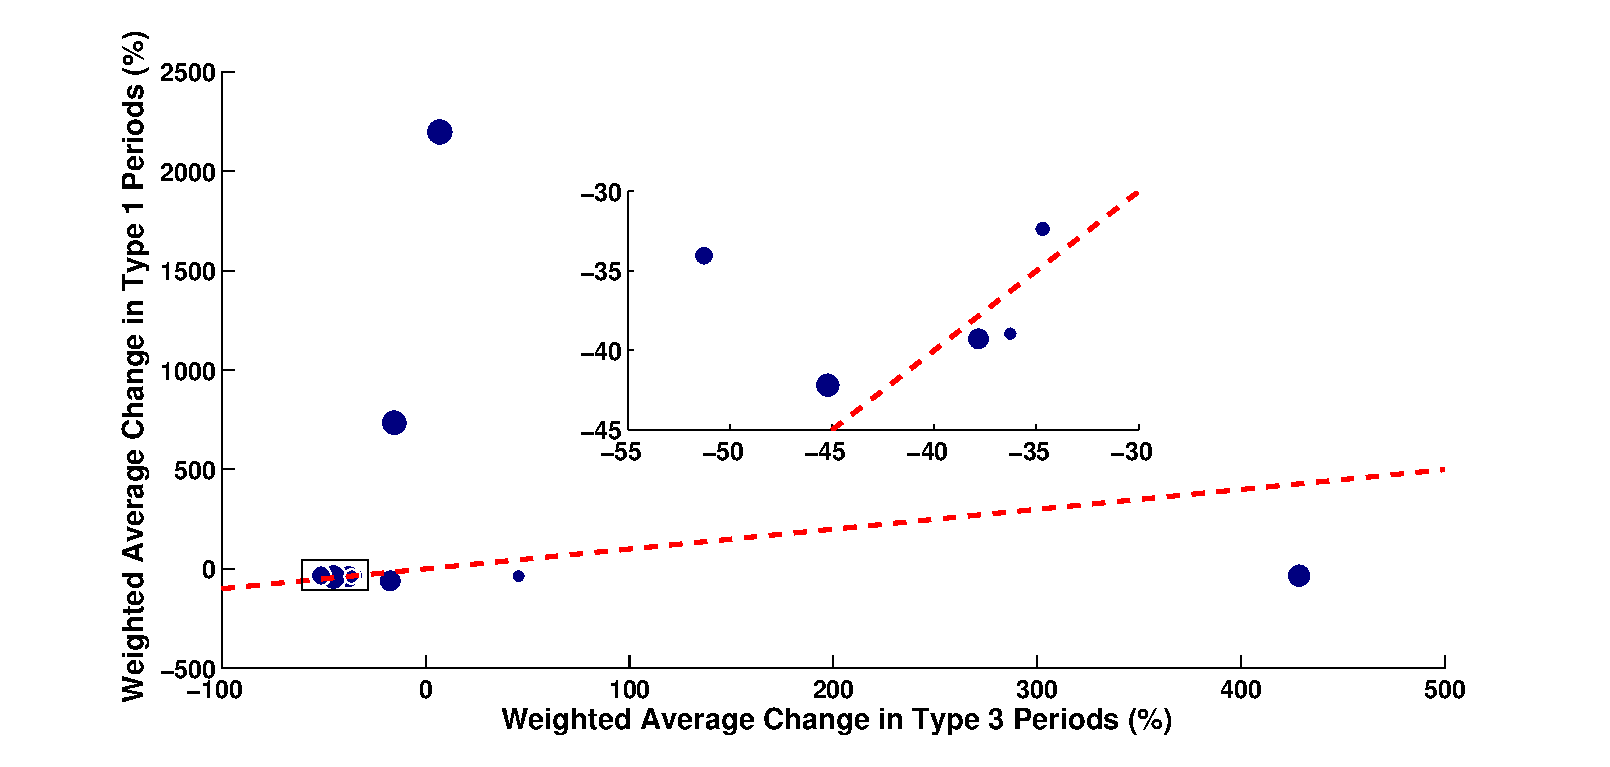
\includegraphics[width = \textwidth]{Figures/OHP_OLP_OHP.eps}
		\caption{Period types 1 and 3.}
	\end{subfigure}
	\hspace{-0.05\textwidth}
	\begin{subfigure}[b]{0.51\textwidth}
		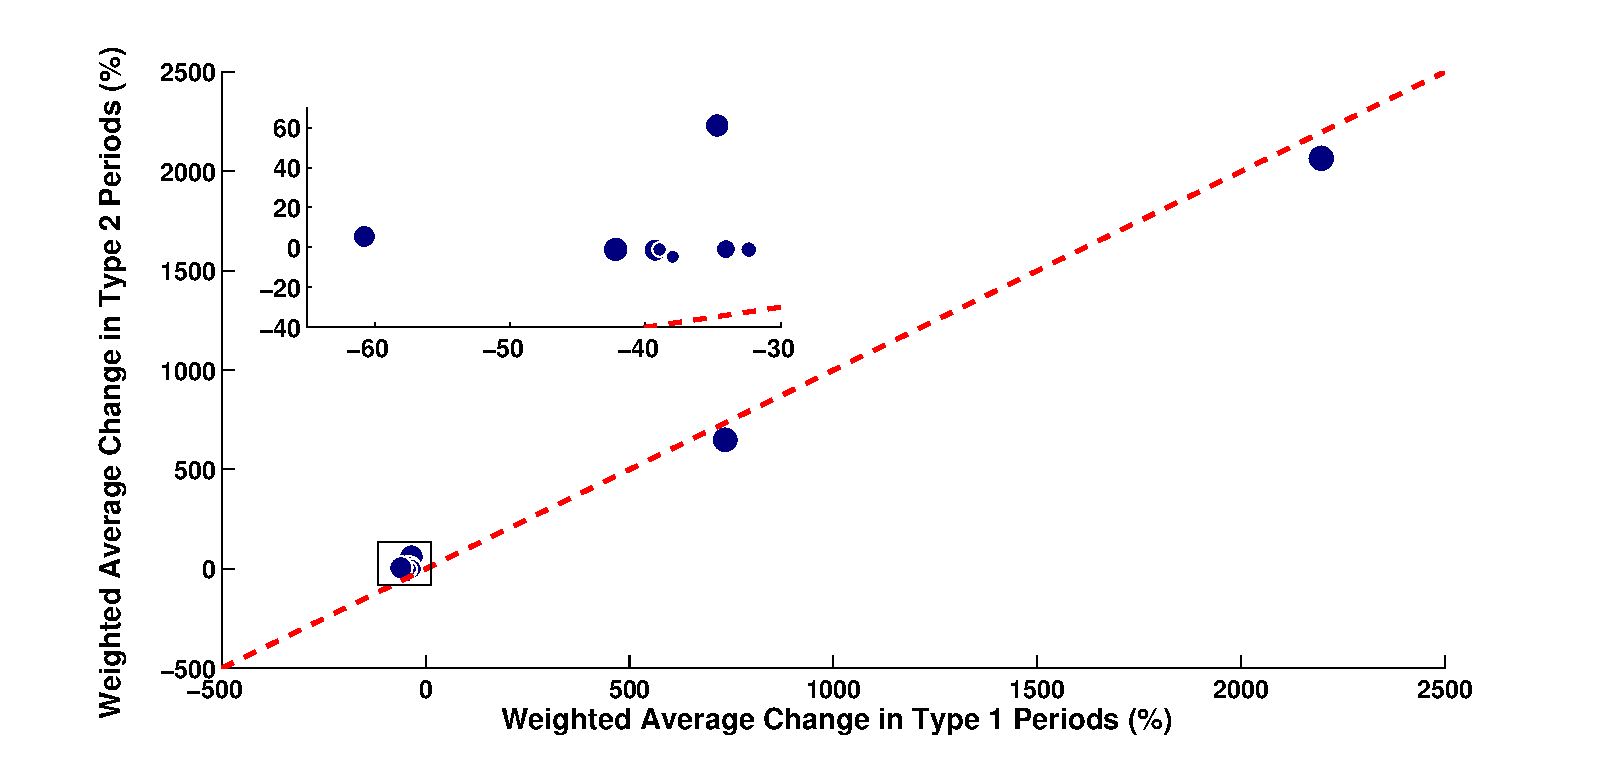
\includegraphics[width = \textwidth]{Figures/OHP_GLP_OLP.eps}
		\caption{Period types 1 and 2.}
	\end{subfigure}
\vspace{-0.1in}
\caption{Average percent changes in usage for the period types in Table \ref{periodtypes}. Users' usage behavior is (a) not affected by the prices when only the numerical discounts, but not the indicator color changes. When (b) both the color and numerical discount change, users increase their usage behavior more in low-price periods.}
\label{fig:OHP_OLP_OHP}
\vspace{-0.1in}
\end{figure*}
Figure \ref{fig:OHP_OLP_OHP}b plots the average change in usage in Type 2 versus Type 1 periods.  The discounts in both periods increased by comparable amounts, but the indicator color changed from orange to green only in Type 2 periods.  Most users' data points lie above the reference line, indicating that usage increased more (or decreased less) in Type 2 as compared to Type 1 periods. Thus, users responded to the indicator color despite the comparable numerical discounts. In fact, 80\% of our participants admitted to this behavior when asked in post-trial interviews whether they paid attention to the indicator color, numerical discounts, or both.

The final stages of the trial offered optimized time-dependent prices, with initial user behavior estimates based on the usage observed in previous stages of the trial with non-optimized prices.  The reduction in peak traffic was measured by the \emph{peak-to-average ratio} (PAR), i.e., the ratio of usage in the peak period to average per-period usage, for each day.  Comparing the PARs from before and after optimized TDP reveals that \emph{optimized time-dependent prices reduce the peak-to-average ratio} from usage before time-dependent prices were offered (time-independent pricing, or TIP).  Moreover, \emph{overall usage significantly increased} after TDP was introduced, partially because people used more in the discounted valley periods. % Valley filling and peak reduction together contributed to lower peak-to-average ratios with TDP.
% Part of this increase is likely due to different times of the year, but we conjecture that the discounts offered with TDP induced people to spend more.

Figure \ref{fig:par}a shows the distribution of daily PARs both before and after TDP was introduced.  The maximum PAR decreases by 30\% with TDP, and approximately 20\% of the PARs before TDP are larger than the maximum PAR with TDP.  Thus, TDP significantly reduced the peak-to-average ratio, flattening demand over the day. Moreover, this decrease in PAR is not due to a net loss of traffic.  Figure \ref{fig:par}b shows the average per-user daily usage observed before and after TDP.  The overall volume of usage after TDP is greater than that before TDP; in fact, across all users, the average change in usage from TIP to TDP is a 130\% increase.  Part of this increase may be due to the time of year--TIP usage was measured from July to September, and the TDP usage in January. TDP, however, is likely a major factor: the discounts during off-peak periods allowed users to consume more data while still spending less money and decreasing the PAR. In fact, in post-trial interviews 30\% of the trial participants admitted to consciously using more data in the heavily discounted periods, with one explicitly comparing the situation to shopping at a clothing sale in department stores.
\begin{figure*}
\centering
	\begin{subfigure}[b]{0.42\textwidth}
		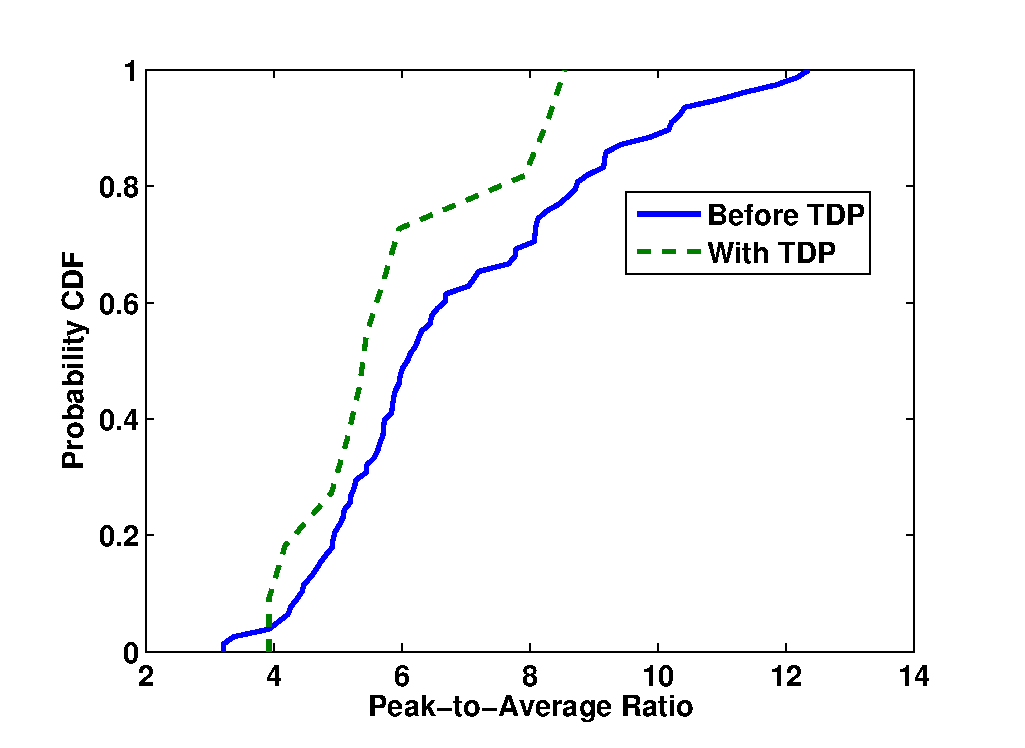
\includegraphics[width = \textwidth]{Figures/PAR.eps}
		\caption{PARs.}
	\end{subfigure}
	\hspace{-0.03\textwidth}
	\begin{subfigure}[b]{0.42\textwidth}
		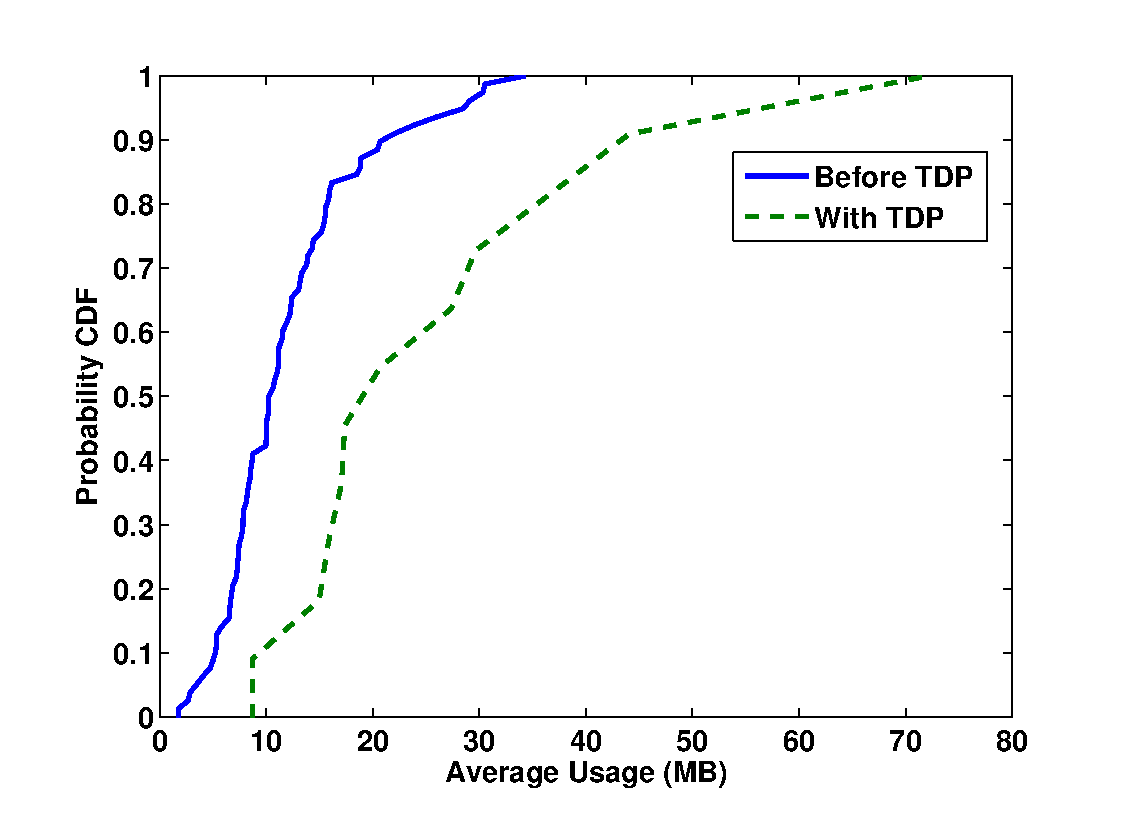
\includegraphics[width = \textwidth]{Figures/Avg.eps}
		\caption{Average daily traffic.}
	\end{subfigure}
\vspace{-0.1in}
\caption{Usage statistics in the TIP (time-independent pricing) and optimized TDP phases of the TUBE trial. When optimized TDP is offered, (a) the ISP's peak-to-average ratio generally decreases, while (b) the average daily traffic per user increases.}
\label{fig:par}
\vspace{-0.1in}
\end{figure*}